% This is "sig-alternate.tex" V2.1 April 2013
% This file should be compiled with V2.5 of "sig-alternate.cls" May 2012
%
% This example file demonstrates the use of the 'sig-alternate.cls'
% V2.5 LaTeX2e document class file. It is for those submitting
% articles to ACM Conference Proceedings WHO DO NOT WISH TO
% STRICTLY ADHERE TO THE SIGS (PUBS-BOARD-ENDORSED) STYLE.
% The 'sig-alternate.cls' file will produce a similar-looking,
% albeit, 'tighter' paper resulting in, invariably, fewer pages.
%
% ----------------------------------------------------------------------------------------------------------------
% This .tex file (and associated .cls V2.5) produces:
%       1) The Permission Statement
%       2) The Conference (location) Info information
%       3) The Copyright Line with ACM data
%       4) NO page numbers
%
% as against the acm_proc_article-sp.cls file which
% DOES NOT produce 1) thru' 3) above.
%
% Using 'sig-alternate.cls' you have control, however, from within
% the source .tex file, over both the CopyrightYear
% (defaulted to 200X) and the ACM Copyright Data
% (defaulted to X-XXXXX-XX-X/XX/XX).
% e.g.
% \CopyrightYear{2007} will cause 2007 to appear in the copyright line.
% \crdata{0-12345-67-8/90/12} will cause 0-12345-67-8/90/12 to appear in the copyright line.
%
% ---------------------------------------------------------------------------------------------------------------
% This .tex source is an example which *does* use
% the .bib file (from which the .bbl file % is produced).
% REMEMBER HOWEVER: After having produced the .bbl file,
% and prior to final submission, you *NEED* to 'insert'
% your .bbl file into your source .tex file so as to provide
% ONE 'self-contained' source file.
%
% ================= IF YOU HAVE QUESTIONS =======================
% Questions regarding the SIGS styles, SIGS policies and
% procedures, Conferences etc. should be sent to
% Adrienne Griscti (griscti@acm.org)
%
% Technical questions _only_ to
% Gerald Murray (murray@hq.acm.org)
% ===============================================================
%
% For tracking purposes - this is V2.0 - May 2012


\documentclass{sig-alternate-05-2015}

%Todd packages and commands
\usepackage[normalem]{ulem} %for sout  
\newcommand{\strikeout}[1]{\sout{#1}}
\newcommand{\quotes}[1]{``#1''}
\newcommand{\q}[1]{``#1''}

\begin{document}

% Copyright
\setcopyright{acmcopyright}
%\setcopyright{acmlicensed}
%\setcopyright{rightsretained}
%\setcopyright{usgov}
%\setcopyright{usgovmixed}
%\setcopyright{cagov}
%\setcopyright{cagovmixed}



% DOI
\doi{10.475/123_4}

% ISBN
\isbn{123-4567-24-567/08/06}

%Conference
\conferenceinfo{PLDI '13}{June 16--19, 2013, Seattle, WA, USA}

\acmPrice{\$15.00}

%
% --- Author Metadata here ---
\conferenceinfo{WOODSTOCK}{'97 El Paso, Texas USA}
%\CopyrightYear{2007} % Allows default copyright year (20XX) to be over-ridden - IF NEED BE.
%\crdata{0-12345-67-8/90/01}  % Allows default copyright data (0-89791-88-6/97/05) to be over-ridden - IF NEED BE.
% --- End of Author Metadata ---

\title{ All Your Code Are Belong to Us \\
Enhancers and Threats to Collective Code Ownership
%Transitioning from \quotes{I Made This!} to \quotes{We Made This!}
}

%
% You need the command \numberofauthors to handle the 'placement
% and alignment' of the authors beneath the title.
%
% For aesthetic reasons, we recommend 'three authors at a time'
% i.e. three 'name/affiliation blocks' be placed beneath the title.
%
% NOTE: You are NOT restricted in how many 'rows' of
% "name/affiliations" may appear. We just ask that you restrict
% the number of 'columns' to three.
%
% Because of the available 'opening page real-estate'
% we ask you to refrain from putting more than six authors
% (two rows with three columns) beneath the article title.
% More than six makes the first-page appear very cluttered indeed.
%
% Use the \alignauthor commands to handle the names
% and affiliations for an 'aesthetic maximum' of six authors.
% Add names, affiliations, addresses for
% the seventh etc. author(s) as the argument for the
% \additionalauthors command.
% These 'additional authors' will be output/set for you
% without further effort on your part as the last section in
% the body of your article BEFORE References or any Appendices.

\numberofauthors{3} %  in this sample file, there are a *total*
% of EIGHT authors. SIX appear on the 'first-page' (for formatting
% reasons) and the remaining two appear in the \additionalauthors section.
%
\author{
% You can go ahead and credit any number of authors here,
% e.g. one 'row of three' or two rows (consisting of one row of three
% and a second row of one, two or three).
%
% The command \alignauthor (no curly braces needed) should
% precede each author name, affiliation/snail-mail address and
% e-mail address. Additionally, tag each line of
% affiliation/address with \affaddr, and tag the
% e-mail address with \email.
%
\alignauthor Todd Sedano\\
       \affaddr{Pivotal}\\
       \affaddr{3495 Deer Creak Road}\\
       \affaddr{Palo Alto, CA}\\
       \email{professor@gmail.com}
\alignauthor Paul Ralph\\
       \affaddr{University of Auckland}\\
       \affaddr{Auckland}\\
       \affaddr{New Zealand}\\
       \email{paul@paulralph.name}
\alignauthor C\'ecile P\'eraire\\
       \affaddr{Carnegie Mellon Unveristy} \\
       \affaddr{Silicon Valley Campus}\\
       \affaddr{Moffett Field, CA 94035, USA}\\
       \email{cecile.peraire@sv.cmu.edu}
}

\date{27 January 2016}

\maketitle
\begin{abstract}

\textit{Context:} Collective code ownership describes the policy that anyone can modify any part of the project. However, simply adopting a policy of collective code ownership is not sufficient for team members to be able to modify any part of the code. 

%A team can adopt a series of policies and practices described in the theory of sustainable software development. 

\textit{Objective:} The purpose of this paper is to understand the factors that foster and decrease a team's sense of collective code ownership.

\textit{Method:} We followed Constructivist Grounded Theory. The primary researcher conducted participant-observation of several software development projects at Pivotal, and interviewed 21 software engineers, designers, and product managers. The researcher iteratively sampled and analyzed until achieving theoretical saturation.

\textit{Results:} A team can use pair programming, overlapping pair rotation, and continuous refactoring to promote collective code ownership. This paper examines how increasing team size, increasing product apathy, increasing team apathy, and increasing code apathy, and breakdowns in pair programming threaten a team's sense of code ownership. 
%The creation of knowledge silos and the accruing of technical debt prevent obstacles for the team to overcome. 

\textit{Limitations:} While the results are highly relevant to Pivotal, the outcomes may not be transferable to other software development organizations with different software development cultures.

\textit{Conclusion:}  Achieving collective code ownership requires significant effort for a team. While the policies and practices align a team towards a high sense of collective code ownership, there are factors that can weaken it. 

\end{abstract}



%
% The code below should be generated by the tool at
% http://dl.acm.org/ccs.cfm
% Please copy and paste the code instead of the example below. 
%
\begin{CCSXML}
<ccs2012>
  <concept>
    <concept_id>10011007.10011074.10011134</concept_id>
    <concept_desc>Software and its engineering~Collaboration in software development</concept_desc>
    <concept_significance>500</concept_significance>
  </concept>
  <concept>
    <concept_id>10011007.10011074.10011092</concept_id>
    <concept_desc>Software and its engineering~Software development techniques</concept_desc>
    <concept_significance>500</concept_significance>
  </concept>
</ccs2012>
\end{CCSXML}

\ccsdesc[500]{Software and its engineering~Collaboration in software development}
\ccsdesc[500]{Software and its engineering~Software development techniques}

%
% End generated code
%


%
%  Use this command to print the description
%
\printccsdesc

% We no longer use \terms command
%\terms{Theory}

\keywords{
Extreme Programming,
Grounded Theory,
Collective code ownership,
Sustainable software development
}


%%
%% Start line numbering here if you want
%%
%%\linenumbers




\section{Introduction}
\textit{Team Code Ownership} (which is similar to \textit{Collective Code Ownership} and \textit{Shared Code}) is a software development practice where any developer on a team has the right to change any of the team’s code. Team code ownership is intended to accelerate development by allowing any developer to fix any team bug and by mitigating delays due to vacations, illness and other absence \cite{ExtremeProgramming2004}.
 
While some research has investigated the effects of different code ownership models, we are unaware of any studies that specifically investigate developers’ sense of team code ownership, that is, the complex interactions between developers’ knowledge, emotions, and approach to code ownership.  

When team code ownership emerged as a core category in a grounded theory study, we therefore exploited this opportunity to investigate factors associated with perceived code ownership and related phenomena. This lead to the following research question. 

\textbf{Research Question:} 

We quickly discovered that having the right to change a file does not mean that a specific developer will feel empowered to and justified in making a specific change. For example, a developer may feel reluctant to change code that he or she does not really understand. As we refined this core finding and allowed it to drive further data collection, we identified five factors associated with feelings of team code ownership. 

This paper consequently reviews existing research connected to team code ownership (Section \ref{RelatedWork}), describes our grounded theory approach (Section \ref{ResearchMethod}), and presents our emerging results: five factors associated with team code ownership (Section \ref{TeamCodeOwnership}). Section \ref{Discussion} discusses the study’s implications and limitations, followed by a summary of its contributions (Section \ref{Conclusion}).
\section{Related Work}
\label{RelatedWork}

\subsection{Team Code Ownership}
In Extreme Programming \cite{ExtremeProgramming2004}, Kent Beck describes a set of interdependent practices for managing feature development and facilitating a collaborative team environment. One of these practices is \textbf{collective ownership}---\quotes{Anyone can change any piece of code in the system at any time.} \cite{ExtremeProgramming2000}. collective ownership is contrasted against \quotes{no ownership} and \quotes{individual ownership.} In 2004, collective ownership is renamed \textbf{shared code} \cite{ExtremeProgramming2004}.

In 2006, Martin Fowler defined \textbf{collective code ownership}, similarly to Beck \cite{FowlerCodeOwnership}, as a contrasting team position to \quotes{strong code ownership} where one person owns each file and \quotes{weak code ownership} where developers can change files, but an owner keeps an eye on files for which they are responsible. 

In 2011, Christian Bird et al \cite{BirdDontTouchMyCode} contrasted the effects of strong- and weak-ownership. They demonstrated that weak ownership leads to more defects than strong ownership for Windows Vista and Windows 7. The study defined ownership for a software component as a percentage of the version control commits for a single developer. They defined a major contributor as someone who has more than 5\% of the git commits. A sensitivity analysis revealed that defining strong code ownership within the range from 2\% to 10\% produced similar results for the study.

In 2015, Brendan Murphy stated that the concept of code ownership must be unpacked and expanded. He argued that the complexities of code ownership are missed by merely examining git commits to determine who modified which files \cite{MurphyIEEESoftware}.

Our paper renames \textbf{collective code ownership} to \textbf{team code ownership}. For small systems and teams, these terms are synonymous. For a large system with multiple teams, in practice, teams would have strong ownership of their portion of the system. The idea that any pair could modify any part of Microsoft Windows or Pivotal Cloud Foundry is impractical.

Team code ownership requires more than a team saying, \quotes{everyone can modify anything.} Instead, this paper examines how a team feels that they own the code. We define \quotes{sense of team code ownership} as the degree to which individual members of the team feel collective ownership.  


\begin{table*}[t]
\renewcommand{\arraystretch}{1.5}
\centering
\caption{Theory of Sustainable Software Development: Principles, Policies, and Practices}
\label{SustainableSoftwareDevelopmentTable}
\begin{tabular}{|p{1.65in}|p{1.35in}|p{1.8in}|p{1.6in}|}
\hline
\multicolumn{4}{|c|}{Sustainable Software Development}                     \\
\hline
Underlying Principles & Policies                  & Removing Knowledge Silos Practices & Caretaking the Code Practices       \\
$\bullet$ Keeping a Positive Attitude Toward Team Disruption & $\bullet$ Team Code Ownership & $\bullet$ Continuous Pair Programming         & $\bullet$  TDD / BDD                   \\
$\bullet$ Encouraging Knowledge Sharing and Continuity & $\bullet$ Shared Schedule           & $\bullet$ Overlapping Pair Rotation & $\bullet$ Continuous Refactoring      \\
$\bullet$ Caring about Code Quality  & $\bullet$ Avoid Technical Debt      & $\bullet$  Knowledge Pollination    & Supported by Live on Master \\ 
\hline
\end{tabular}
\end{table*}

\subsection{Theory of Sustainable Software Development}
\label{SustainableSoftwareDevelopmentTheory}
We describe the theory of Sustainable Software Development through Team Code Ownership in paper by the same name \cite{SustainableSoftwareDevelopment} and summarize it in Table \ref{SustainableSoftwareDevelopmentTable}. The theory describes how teams can continue to deliver value in spite of team disruptions. The theory is a collection of synergistic principles, policies, and practices encouraging a positive attitude towards team disruption, knowledge sharing and continuity, as well as caring about code quality. The practices actively remove knowledge silos and caretake the code so that any pair can work on any story in the backlog. 

\subsection{Psychological Ownership}
Psychological ownership refers to \quotes{the feeling of possessiveness and of being psychologically tied to an object} \cite{Pierce2001}. Targets of ownership, whether physical or immaterial, become the extension of one’s self. \quotes{what is mine becomes (in my feelings) part of ME} \cite{Isaacs1933}. Ownership can be attached to a part or the whole. Psychological ownership occurs when the object becomes part of the psychological owner’s identity. Psychological ownership answers the question, \quotes{What do I feel is mine?}

Changes in ownership can have strong effects on our self-identity. An augment in possessions can produce positive effects \cite{Formanek1994}, while a diminish can lead to a personality shrinkage \cite{James1890}. Someone threatening a person’s ownership can trigger strong emotions and responses.

Peirce \cite{Pierce2001} identifies three sources or \quotes{roots} of psychological ownership: efficacy and effectance, self-identity, and having a place. A major reason for possession of physical goods or abstract ideas is rooted in the innate human desire to be in control; being able to alter one’s environment creates feelings of efficacy and pleasure. Ownership fulfills the need for self-identification as people define themselves, express themselves, and ensure their own survival by what they own. Ownership fulfills the need to have a place and a territory to possess. \quotes{Each motive facilitates the development of psychological ownership, rather than directly causes this state to occur.} Psychological ownership occurs with code because creating software can satisfy the desire for efficacy and effectance, self-identity, and having a place.

Peirce identifies three paths or \quotes{routes} to ownership: controlling the target, coming to intimately know the target, and investing the self into the target. With \emphasis{controlling the target}, targets that can be controlled are perceived to be part of the self.  As  individuals repeatedly exercise control of an object, eventually this leads to \quotes{feelings of ownership toward that object.} The higher the autonomy of the job task, the more likely ownership develops toward the activity. When a person has little control over an activity, psychological ownership is unlikely to develop. With \emphasis{coming to intimately know the target}, the association with the object creates feelings of ownership. One example is when a gardener feels that the garden belongs to the gardener. (This happens routinely with software developers who feel that they own part of the code base, when in reality, the company owns the software.) Feelings of ownership increase as one becomes intimately familiar with the object and associated with it. With \quotes{investing the self into the target,} we feel that we own what we create, shape or produce. Spending time, energy, and effort enables us to alter our view of ourselves to include identity with the object. The more investing in the object, the stronger the psychological ownership. Nonroutine, complex jobs infuse more of our own ideas resulting in increased ownership.

\section{Research Method}
\label{ResearchMethod}

\subsection{Constructivist Grounded Theory}
We followed Charmaz' approach to Grounded Theory \cite{Charmaz}, which provides an iterative approach to data collection, data coding, and analysis resulting in an emergent theory. The two primary data sources were field notes collected during continuous participant observations of a 7.5 month project and interviews with 21 Pivotal software engineers, interaction designers, and product managers. Interviews were recorded, transcribed, coded, and analyzed using constant comparison. Our presentation is informed by Stol et al.’s reporting guidelines for grounded theory studies in software engineering \cite{StolGTinSE}. 

When starting a grounded theory research study, the core question is \quotes{What is happening here?} (Glaser, 1978) \cite{GlaserTheoreticalSensitivity}. Our initial core question was: \quotes{What is happening at Pivotal when it comes to software development?} This question led to the Theory of Sustainable Software Development summarized in Section \ref{SustainableSoftwareDevelopmentTheory}. When team code ownership emerged as one of the core categories of the theory, the researcher collected additional data in order to identify the factors affecting the sense of code ownership. These factors are introduced in Section \ref{TeamCodeOwnership} and are the main contributions of the paper.

\subsection{Data Collection}
The primary researcher relied on \quotes{intensive interviews,} which Charmaz summarizes as \quotes{open-ended yet directed, shaped yet emergent, and paced yet unrestricted} \cite{Charmaz}. The technique relies on open-ended questions. The purpose is for the researcher to enter into the participant's personal perspective within the context of the research question. 

While exploring new emergent core categories, whenever possible, the researcher initiated subsequent interviews with a goal of not forcing the issue. For example, \quotes{please draw your feelings about the code} often resulted in conversations about code ownership. After the interview, the interview was transcribed into a Word document with timecode stamps for each segment.

The primary researcher also collected field notes while working as an engineer. The field notes comprise of multiple paragraph entries recorded several times a week collected over a six month period. The field notes describe individual and collective actions, captures what participants defined as interesting or problematic, and include anecdotes and observations. 

\subsection{Research Context: Pivotal}
\label{ResearchContext}
Pivotal is a large American company with 16 offices around the world. One of its divisions is Pivotal Labs. Pivotal Lab's mission is to both deliver highly-crafted software products and provide a transformative experience for their client's engineering cultures. To change a developer's way of working, Pivotal combines the client's software engineers with Pivotal's engineers at a Pivotal office where they can experience Extreme Programming in an environment conducive for agile development. For startups, Pivotal might be the first engineers working on the project. For enterprise clients, Pivotal provides additional engineering resources to accomplish new business goals. 

Common team sizes are six developers plus an interaction designer and a product manager. In the history of the Palo Alto office, the number of developers on a project ranges from 2 to 28. Larger projects are organized into smaller coordinating teams with one product manager per team and one or two interaction designers per team.

Commonly utilized technologies include Angular, Android, backbone, iOS, Java, Rails, React, and Spring often deployed onto Pivotal's Cloud Foundry. 

Pivotal Labs has followed Extreme Programming \cite{ExtremeProgramming2004} since the late 1990's. While each team is autonomous in making its own decisions as to what is best for a particular project, the company culture strongly suggests following all of the core practices of Extreme Programming. This includes Pair Programming, Test Driven Development, Weekly Retrospectives, Daily Stand-ups, Prioritized Backlog, Whole Team ownership of the project and code base, plus Kanban's notion of work flowing through people.

\section{Team Code Ownership}
\label{TeamCodeOwnership}

In the literature, collective code ownership is often treated as a policy statement. In this case, simply claiming that \quotes{anyone can modify any piece the code} was not sufficient to engender willingness to modify any file. Rather, ownership is an emotional or qualitative attribute that ties all developers on the team to the project and code base. It is a spectrum where, on one side, each individual has ownership of only their code, and on the other side, everyone on the team owns the entire code base. Some events appear to erode the team's sense of ownership over the project’s duration, while some practices appear to counteract these erosions (next). This section details the five factors that appear most related to team code ownership and examples of events or tendencies that erode it (Table \ref{TeamCodeOwnerhipFactors}). 

\begin{table}[]
\renewcommand{\arraystretch}{1.5}
\centering
\caption{Factors affecting Team Code Ownership}
\label{TeamCodeOwnerhipFactors}
\begin{tabular}{|p{3.1in}|}
\hline
System Context \\
Code Contribution \\
Code Quality \\
Product Quality \\
Team Cohesion \\
\hline
\end{tabular}
\end{table}

\subsection{System Context}
\textbf{Definition:} System context is the knowledge and situational awareness about the code, including the discourse that surrounds the code. System context includes understanding existing design decisions, underlying technologies, the relationship between features and user needs, and how existing features have been implemented.

\textbf{Purpose:} Developing a deep knowledge of the system exercises the \quotes{intimately knowing the target} path of psychological ownership.

For a pair to work efficiently on any part of the system, one of them needs to have enough context to know how that part of the system works. Without enough context, a pair might struggle, slow down, or be blocked in working on a feature.

Code ownership seems to vary with the context that the developer has about the code; the more the developer knows, the higher the sense of ownership. The size of the code base or the number of developers working in parallel can make it difficult for a programmer to develop a deep system context level.

\textbf{Threat: Increasing code base size.} The primary researcher participated on a team working with a large code base that was over eight years old and the team did not have a full understanding of the system. Initially, the team felt little ownership of the code, even though the team was responsible for it and agreed to \singleQuote{team code ownership.} Often the team would need to ask a product manager why certain features existed in the code to understand what the code was trying to do. In time, as the team worked with the code and gained context, the team’s sense of ownership improved.

\textbf{Threat: Increasing team size.} The primary researcher observed the relationship between team size and code context on five Pivotal projects as a participant-observer. As team size increases, the ability to gain system context decreases. Every day, all pairs are adding to the system. On a five pair team, so much work is happening each day that it becomes increasingly difficult to keep track of everything that changes.

One developer on a ten-person project said, \participantQuote{I feel that we don't have the context spread around fully. Having five, sometimes six, pairs on the project makes it go really fast, so it's hard to keep context.}

When developers do not have context about part of a system, or context about what remains to be done to finish a story, reluctance to start the next story at the top of the backlog emerges. It’s easier to start a story that touches part of the system that they know. As one developer reflected, \participantQuote{I am not completely comfortable to jump into stories on certain aspects [of the system].}

As a coping strategy, one developer, before the start of the work day, skimmed the git commits from the previous day to learn about new classes and changes in design, and to understand the features the team added. Another potential mitigation strategy is for each pair of the team to start the pairing day by reviewing changes from the previous day. For a large team, this additional work becomes increasingly necessary. 

As team size grows, there is a potential risk of decreasing an individual developer’s sense of team code ownership. 

\subsection{Code Contribution}
\textbf{Definition:} Code contribution is the portion of the code that a given developer has worked on. 

\textbf{Purpose:} Personally contributing to the code base increases a developer’s sense of ownership by exercising \quotes{investing in the target} path of psychological ownership. As a developer works on the code base, the developer’s system context level increases. While code contribution level influences the system context level, it is not necessary related: developers might learn about the code through other means different from direct contribution, including conversations at stand-up, impromptu team huddles, or a pair saying \participantQuote{Check out what we did yesterday.}

\textbf{Threat: Inability to contribute.}  A developer’s inability to contribute to the code base decreases the developer’s sense of ownership. 

This could happen, for instance, during a pair programming breakdown. When the pairing experience breaks down, one person drives the code development while the partner passively watches. (We call this dynamic \quotes{Performance Pair Programming,} when one developer plows through a story and stops listening to the developer’s partner.)  When one person is writing all the code, individual code ownership replaces team code ownership.  

In one situation, the partner took over and ignored the participant’s input. The participant reflected, \participantQuote{I did not understand what was really going on. I wouldn't be able to explain deeply what we had done. I wouldn't be able to maintain it. I didn't really write it, so I feel very little ownership of it.} 

Ideally, Pair Programming is a collaborative experience where both individuals are unable to tell who wrote which portions of the code. 

\subsection{Code Quality}
\textbf{Definition:} Code quality relates to how well the code satisfies the project’s desirable quality attributes. Desirable quality attributes might include design qualities (e.g. conceptual integrity, maintainability, reusability, discoverability), run-time behavior (e.g. availability, interoperability, manageability, performance, reliability, scalability, security), system qualities (e.g. supportability, testability), and user qualities (e.g. usability) \cite{Meier2009}. 

\textbf{Purpose:} How well the code satisfies the project’s desirable quality attributes affects the team’s sense of ownership. When a product does not achieve an acceptable quality level, a developer may not want to be identified with the product and thus the self-identification motivation of psychological ownership is not being met. Low quality products also tend to involve a disproportionate amount of bug fixes. Developers need a balance between creating new features and fixing bugs each week. Working only on bugs for weeks affects their sense of ownership.    

\textbf{Threat: Pressure to deliver and deprioritizing continuous refactoring.} When developers are pressured to deliver more features at the expense of Continuous Refactoring, the code acquires technical debt, the code becomes harder to work with, and developers can begin to feel apathetic about the code. When developers begin to experience code apathy, this decreases their sense of team code ownership. 

When refactoring is neglected, new code is simply bolted onto the existing design. Each time the team bolts something else on, it gets more difficult to bolt on the next piece. Thus, a dilemma arises for the programmers working on the next story that touches this part of the code: do they continue bolting on more code, or do they perform the pretermitted refactoring? When the team begins avoiding refactoring, it's a sign that code apathy may be settling in. Code apathy results in reduced quality, as the developers become less invested in the craftsmanship of the code.

One developer felt \participantQuote{proud and disgusted} about the code base. He is simultaneously proud of each refactoring that the team performed and disgusted by the technical debt the team accrued by taking shortcuts to ship more features. The developer drew Figure \ref{Programmer1} to shows his feeling about the code, \participantQuote{It is generally orderly with a few bits that maybe are not as orderly.}

Before the first launch of a product, the product manager suggested that the team deliver more features at the expense of technical debt. For some of the team, this was an unacceptable tradeoff, and those developers decided not to cut corners. Others on the team complied with the request and incurred technical debt. The entire team ended up paying the consequences with extensive refactors after the launch. On a communal code base, one pair adding tech debt affects everyone on the team.

When code apathy settles in, team members adopt the attitude that someone else will solve the problem with the code. When this attitude permeates a team, no one is solving the problems. 

\begin{figure}[t]
\centering
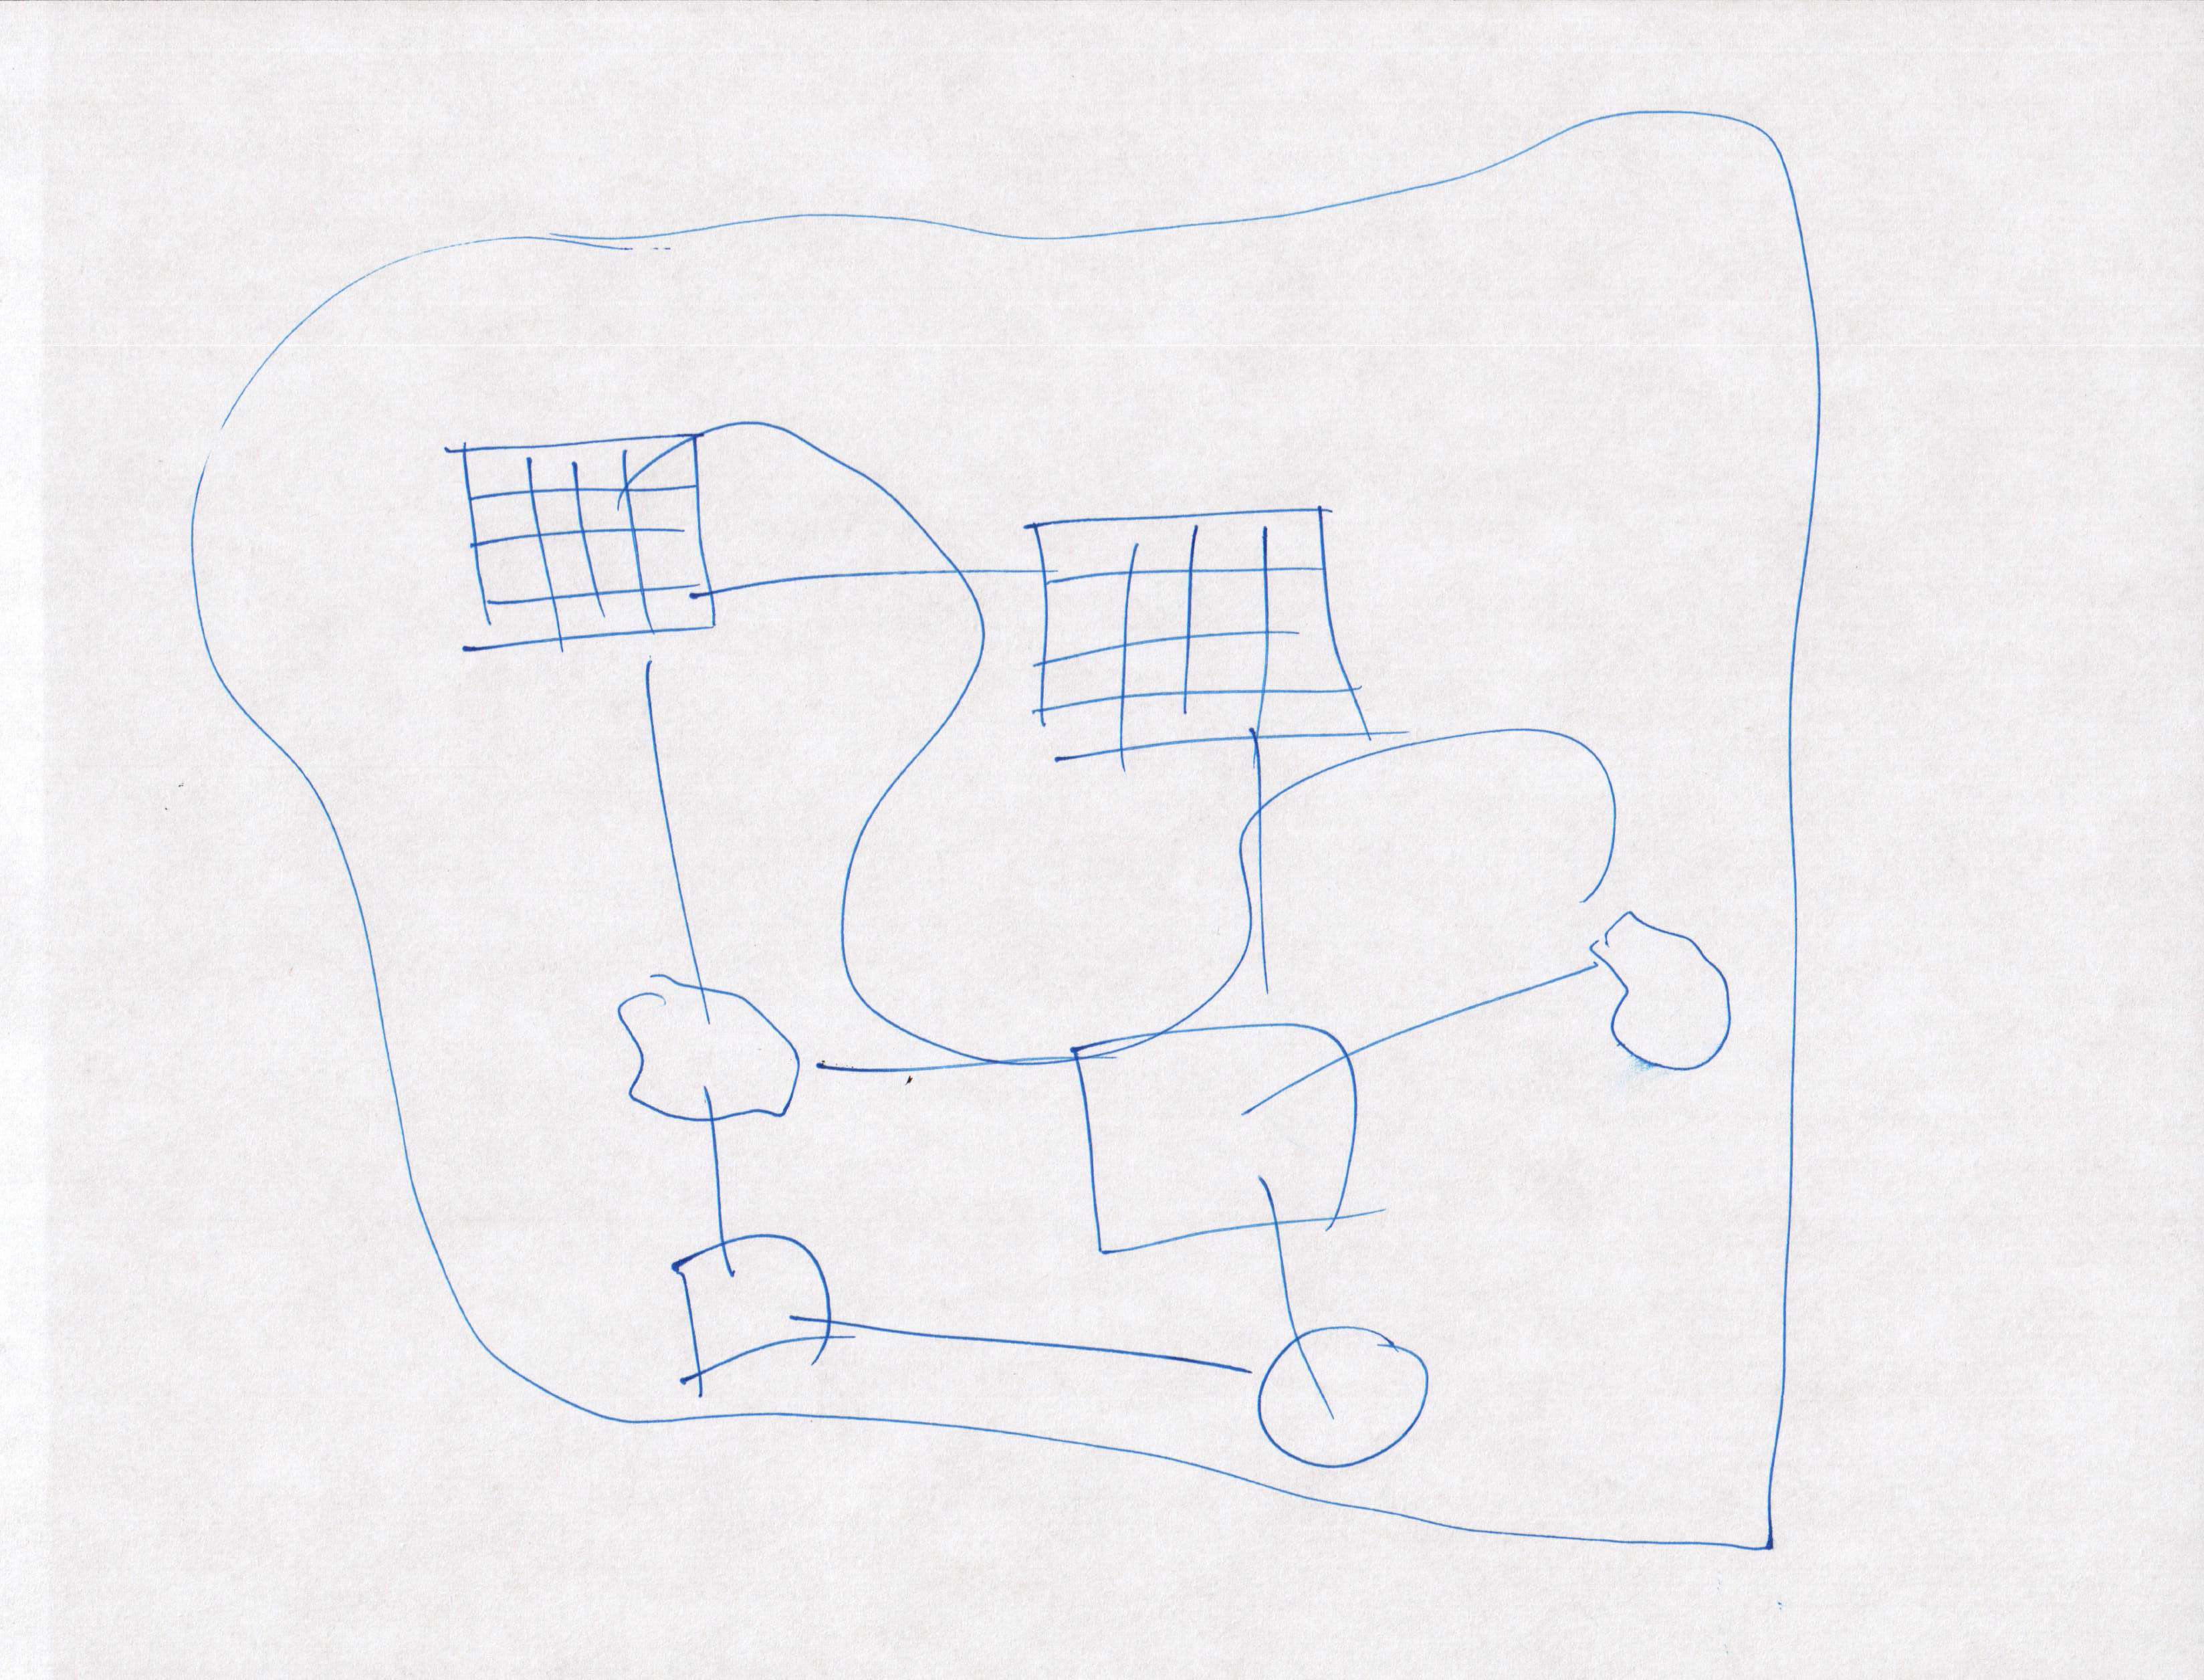
\includegraphics[width=3.45in]{team_code_ownership_images/CodeOwnership.jpg}
\caption{\quotes{Draw how you feel about the code}}
\label{Programmer1}
\end{figure}

The team wants to feel \quotes{pride in improving code quality.}  It feels good to be improving the code design and readability. If the team starts neglecting these concerns, it can engender a sense of disgust and an apathy for the code can spread throughout the team.

\subsection{Product Quality}
\textbf{Definition:} Product quality is believing that the product will satisfy the user’s needs.

\textbf{Purpose:} Engineers want to create products that matter to the user. Delivering a product that matters to someone satisfies the self-identity motivation of psychological ownership.

\textbf{Threat: Ignoring developers feedback about the product.} Product apathy occurs when a developer loses investment in the features of the product. Pivotal’s balanced team approach is founded on collaboration between product managers, interaction designers, and developers. When product managers, or other stakeholders, ignore feedback from developers, developers can begin to feel less ownership in the product, and in turn be less motivated to work on the project. 

When picking up a story, a developer verifies that the story contains clear acceptance criteria. In the absence of acceptance criteria, the developer typically clarifies with the product manager what must be done. On one project when the stakeholders were ignoring feedback from the developers, one developer recalled, \participantQuote{In this case, I don't feel like spending the extra energy to go and say, `Hey, are you sure? Is this what you want?'} 

Product apathy can result in a poorly crafted product that does not meet the customer’s needs.

\subsection{Team Cohesion}
\textbf{Definition:} Team cohesion is the degree to which team members identify as part of the team, stick together through adversity and take pride in the team’s accomplishments \cite{Bollen1990Perceived, Beal2003Cohesion, Whitworth2007Motivation}.

\textbf{Purpose:} Team cohesion satisfies the \quotes{having a place} motivation of psychological ownership.

\textbf{Threat: Distancing a developer from the team.} Team apathy manifests when developers do not feel that they are a part of the team. It is hard to feel team ownership of the code base when one feels excluded from the team.

We observed several behaviors that can distance a developer from the team: interrupting the developer during discussions, using poor listening skills so that the developer feels unheard, or talking beyond the developer’s level of technical expertise. 

On one team, during discussions, the team talked about code but never looked at the source code. For one visual learner, it was hard for the programmer to follow the discussions. Sometimes the team discussed parts of the code that the individual had not seen recently. When the team discussed two variants of coding practices without showing concrete examples, the programmer could not contribute. When the developer raised this issue to the team and the team continued with the status quo, the programmer felt marginalized by the team.

Poor onboarding of developers can contribute to feeling of isolation. On one project, there was a time crunch and the team was feeling the pressure to deliver stories. When the team added developers, the team had a \quotes{sink or swim} attitude, letting new team members figure things out own their own, hence making them feel unwelcome.

When developers feel that the team does not care about them, their sense of ownership can decrease.

\section{Discussion}
\label{Discussion}
\subsection{Transitioning to team code ownership}
\label{Transitioning}

The above results have numerous implications for teams attempting to transition to team code ownership. 

Some developers effortlessly make the transition to team code ownership. They immediately see the benefits of being able to modify any part of the code base and quickly shift from \participantQuote{I made this} (personal ownership) to \participantQuote{we made this} (collective ownership.)

Others may struggle with team code ownership for several reasons:

\begin{itemize}  

\item Developers may struggle to transition to a caretaker mindset.  In one interview, a software engineer struggled to describe the developer’s relationship with the code on a very challenging project and settled in on the caretaker metaphor: \participantQuote{Sometimes I kind of feel like a janitor to [the code base].  Maybe caretaker would be better. Yeah, probably caretaker. I feel like a janitor just cleans up messes, but a caretaker makes things better.} 

\item A developer may be distraught at \participantQuote{seeing my work slowly removed from the app.} 

\item Developers can no longer take pride in functionality that they exclusively develop.

\item Existing knowledge silos, which hinder team code ownership, may be slow to break down.
 
\end{itemize}

New hires struggling with the transition slowly realize that \participantQuote{Someone else is going to take over and they're going to do fine. I can move onto something else and that’s okay.} They recognize the lack of long-term individual authorship, learn to expect their code to be transitory, develop trust in their teammates and thus loosely hold personal contributions. \participantQuote{The code that I write today may be in the code base for a little while, and it will evolve into something better.} Eventually  they experience the benefits of a collaborative environment: \participantQuote{People are a lot more flexible all across the board, with changing things or accepting feedback or collaborating,} and the team can say \participantQuote{Hey, this is our code!}

Shifting from individual to team code ownership may requires multiple and complementary practices to actively remove knowledge silos. In this case, daily pair rotation helped combat knowledge silos. Moreover, for developers with strong individual ownership tendencies, sharing ownership first with a small group (where trust and communication come easier) may help. One Pivotal engineer uses improvisation and collaboration games to help teams practice letting go of control, trusting the team, and learning to be pleasantly surprised by what emerges. 

\subsection{Results Evaluation}

The factors influencing team code ownership presented in Section \ref{TeamCodeOwnership}, have emerged from the Grounded Theory research study introduced in Section \ref{SustainableSoftwareDevelopmentTheory}. While other factors may influence team code ownership, we focus only on those that were observed during the study. Grounded Theory studies can be evaluated using the following criteria \cite{Charmaz}: 

\textbf{Credibility:}  The 21 intensive open-ended interviews and numerous field notes from participant-observation serve as a rich and credible data set for the analysis. 

\textbf{Originality:} The paper broadens the idea of team code ownership by acknowledging that collective code ownership is more than a policy statement, and by uniquely identifying factors that affect the team’s sense of code ownership.

\textbf{Resonance:} Several participants reviewed our findings and indicated that both the factors and threats resonate with their experience.

\textbf{Usefulness:} The study identifies factors associated with ownership and suggests several ways of engendering team code ownership.

This work analyzed software projects at the Silicon Valley office of Pivotal following Extreme Programming. From an \textbf{external validity} perspective, grounded theory is non-statistical, non-sampling research. Our results therefore cannot be statistically generalized to a population. Rather, researchers and professionals can adapt the concepts and ideas to other contexts case-by-case. 

Finally, our results might be influenced by \textbf{researcher bias} or \textbf{prior knowledge bias}. A risk of the participant-observer technique is that the researcher may lose perspective and become biased by being a member of the team. While a participant-observer gains perspective an outsider cannot, an outside observer might see something a participant observer will miss. Similarly, while prior knowledge helps the researcher interpret events and select lines of inquiry, prior knowledge may also blind the researcher to alternative explanations \cite{GlaserIssues}. 
We mitigated these risks by recording interviews and having the second and third authors review the coding process. 

\section{Conclusion}
\label{Conclusion}
This paper reports results from a participant-observation, constructivist grounded theory study of Pivotal, a large America software company employing Extreme Programming practices. It provides three main contributions.

1) Our observations clearly indicate that \textbf{team code ownership is a feeling to be engendered not a policy to be decreed}.

2) Meanwhile, both discussions with and observations of participants suggest five factors associated with strong feelings team code ownership. Pivotal developers more acutely feel team code ownership when 1) they understand the system context; 2) they contribute to the code in question; 3) they perceive code quality is high, 4) they engage with the product, and 5) they perceive team cohesion is high.   

3) Moreover, diverse events and trends can undermine sense of ownership, including:  increasing code base size, increasing team size, inability to contribute, pressure to deliver and prioritize continuous refactoring, ignoring developers feedback on product, and distancing a developer from the team. 

In conclusion, Pivotal’s developers find team code ownership highly advantageous; however, transitioning to a team code ownership model is easier for some than others. Some agile practices including continuous pair programming, overlapping pair rotation, continuous refactoring, and testing appear to help. Promising angles for future research include more nuanced explorations of the code ownership spectrum, further exploration of the roles of emotion and identity, as well as developing specific practices for facilitating ownership transitions. 

\section{Acknowledgement}
Thank you to Rob Mee, David Goudreau, Ryan Richard, and Zach Larson for making this research possible.













% \begin{table*}[]
% \centering
% \caption{Sense of collective code ownership}
% \label{Sense}
% \begin{tabular}{p{1.5in}p{5.6in}}

% transitioning into         & onboarding developers switch from \quotes{I made this} (personal ownership) to \quotes{we made this} (communal ownership) pride in workmanship \\ \hline
% fundamental attitude       & enabled by loosely holding personal contributions and recognizing lack of long term individual authorship                                          \\ \hline
% enabled by                 & Sustainable Software Development practices                                                                                                         \\ \hline
% eroded by                  & product apathy,                                                                                                                                    \\
%                           & large team size,                                                                                                                                   \\
%                           & team apathy,                                                                                                                                       \\
%                           & - stakeholders not listening to feedback                                                                                                           \\
%                           & - not understanding why decisions are made                                                                                                         \\
%                           & - not understanding the plan                                                                                                                       \\
%                           & - person burning out                                                                                                                               \\
%                           & code apathy,                                                                                                                                       \\
%                           & low code understanding,                                                                                                                            \\
%                           & assigning blame for mistakes,                                                                                                                      \\
%                           & getting easily blocked,                                                                                                                            \\
%                           & poor onboarding of developers                                                                                                                      \\
%                           & leaving people behind (performance programming)                                                                                                    \\
%                           & personal goals not aligned with team goals                                                                                                         \\
%                           & technical debt                                                                                                                                     \\
% \hline
% signs of healthy ownership & wanting to do the right thing  \\
%                           & sense of caring                                                                                                                                    \\
%                           &                                                                                                                                                    \\
%                           &                                                                                                                                                    \\
%                           &                                                                                                                                                    \\
%                           &                                                                                                                                                    \\
%                           &                                                                                                                                                   
% \end{tabular}
% \end{table*}






% The following two commands are all you need in the
% initial runs of your .tex file to
% produce the bibliography for the citations in your paper.
\bibliographystyle{abbrv}
\bibliography{bibliography}  % sigproc.bib is the name of the Bibliography in this case
% You must have a proper ".bib" file
%  and remember to run:
% latex bibtex latex latex
% to resolve all references
%
% ACM needs 'a single self-contained file'!
%

% That's all folks!
\end{document}

